\documentclass[12pt,letterpaper]{article}
\usepackage[utf8]{inputenc}
\usepackage{amsmath}
\usepackage{amsfonts}
\usepackage{amssymb}
\usepackage{fancyhdr}
\usepackage{graphicx}
\usepackage[left=0.79in, right=0.79in, top=0.79in, bottom=0.79in]{geometry}
\usepackage{listings}
\usepackage[svgnames]{xcolor}
\author{Chathan Driehuys}

\definecolor{diffstart}{named}{Grey}
\definecolor{diffincl}{named}{Green}
\definecolor{diffrem}{named}{OrangeRed}

\lstdefinelanguage{diff}{
	basicstyle=\ttfamily\small,
	morecomment=[f][\color{diffstart}]{@@},
	morecomment=[f][\color{diffincl}]{+},
	morecomment=[f][\color{diffrem}]{-},
}

\lstset{frame=tb,
	language=html,
	aboveskip=3mm,
	belowskip=3mm,
	showstringspaces=false,
	columns=flexible,
	basicstyle={\small\ttfamily},
	breaklines=true,
	breakatwhitespace=true,
	tabsize=2
}

\graphicspath{{./images/}}

\pagestyle{fancy}
\lhead{COMP 535}
\chead{Firewall}
\rhead{Chathan Driehuys}

\begin{document}
	\noindent \textbf{UNC Honor Pledge:} I certify that no unauthorized assistance has been received or given in the completion of this work.
	
	\vspace{.5in}
	
	\section*{Prerequisites}
		In order to demonstrate the effect of firewalls, we first had to set up two virtual machines (VMs) on the same network. To prove that the two machines can exchange traffic, we can show the result of pinging one machine from another.
		
		\begin{figure}[h]
			\begin{center}
				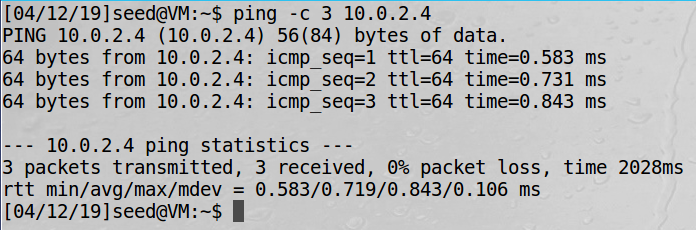
\includegraphics[width=4in]{task-0-ping}
			\end{center}
			\caption{The result of pinging one virtual machine from another.}
			\label{fig:task-0-ping}
		\end{figure}
	
	\section*{Task 1}
		Using the set of rules shown in Figure \ref{fig:task-1-ufw-rules}, we can block the following operations:
		
		\begin{enumerate}
			\item Telnet from A to B
			\item Telnet from B to A
			\item Access to \texttt{example.com} from A
		\end{enumerate}
		
		\begin{figure}
			\begin{center}
				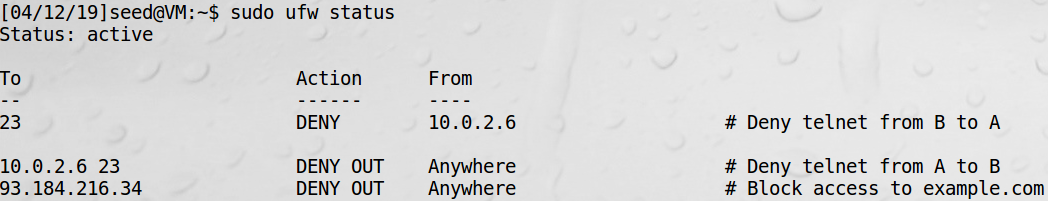
\includegraphics[width=\linewidth]{task-1-ufw-rules}
			\end{center}
			\caption{The \texttt{ufw} rules for task 1.}
			\label{fig:task-1-ufw-rules}
		\end{figure}
		
\end{document}